\chapter{A Top down view of the architecture}
\label{architecure}




\begin{figure}[!htbp]
\centering
\captionsetup{justification=centering}
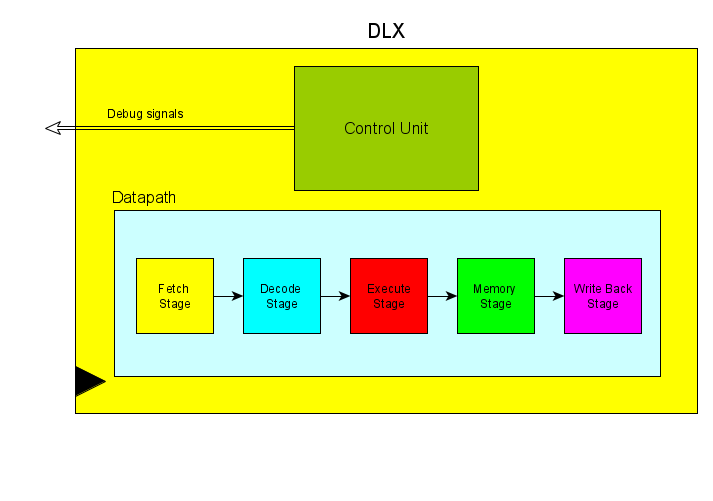
\includegraphics[scale=0.4,angle=0]{./chapters/figures/dlx_top.png}
\caption{DLX top level entity}
\label{fig:dlxarch}
\end{figure}


\section{Control Unit}



\begin{figure}[!htbp]
\centering
\captionsetup{justification=centering}
%\includegraphics[scale=0.35,angle=0]{./figure/graphs/utilization_factor_30mhz_int16.pdf}
\caption{State Diagram}
\label{fig:statediag}
\end{figure}


\section{Datapath}



\begin{figure}[!htbp]
\centering
\captionsetup{justification=centering}
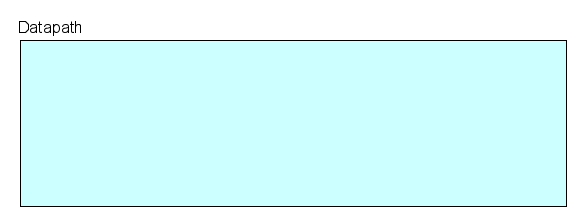
\includegraphics[scale=0.4,angle=0]{./chapters/figures/datapath.png}
\caption{Datapath}
\label{fig:dp}
\end{figure}